\section{Analyse von Geschäftsprozessen}

\subsection{Ziele und Methoden der Prozessanalyse}
    \subsubsection*{Ziele}
        Das systematische Aufspüren von Schwachstellen und Verbesserungspotentialen zur kontinuierlichen Verbesserung der Prozesse.
    \subsubsection*{Methoden}
        Unterscheidung zwischen qualitativen und quantitativen Analyseansätzen. Qualitative Methoden umfassen eine methodische Vorgehensweise zur Problemerkennung, während quantitative Methoden analytisch vorgehen und auf Rechenwerken basieren.

\subsection{Wertschöpfungsanalyse}
    Kunden eines Prozesses sind jene die einen Vorteil durch die Ausführung einen Prozess haben (interne oder externe Kunden eines Prozesses)
    \subsubsection*{Zerlegung der Aktivitäten}
        Aktivitäten eines Prozesses in Schritte unterteilen, danach bewerten (Wertschöpfend, Geschäftsförderlich, nicht-Wertschöpfend)
    \subsubsection*{Eliminierung ineffizienter Schritte}
        Nicht-wertschöpfende Schritte sollen eliminiert oder automatisiert werden

\subsection{Ursachen-Wirkungsdiagramm}
    \begin{figure}[ht]
        \centering
        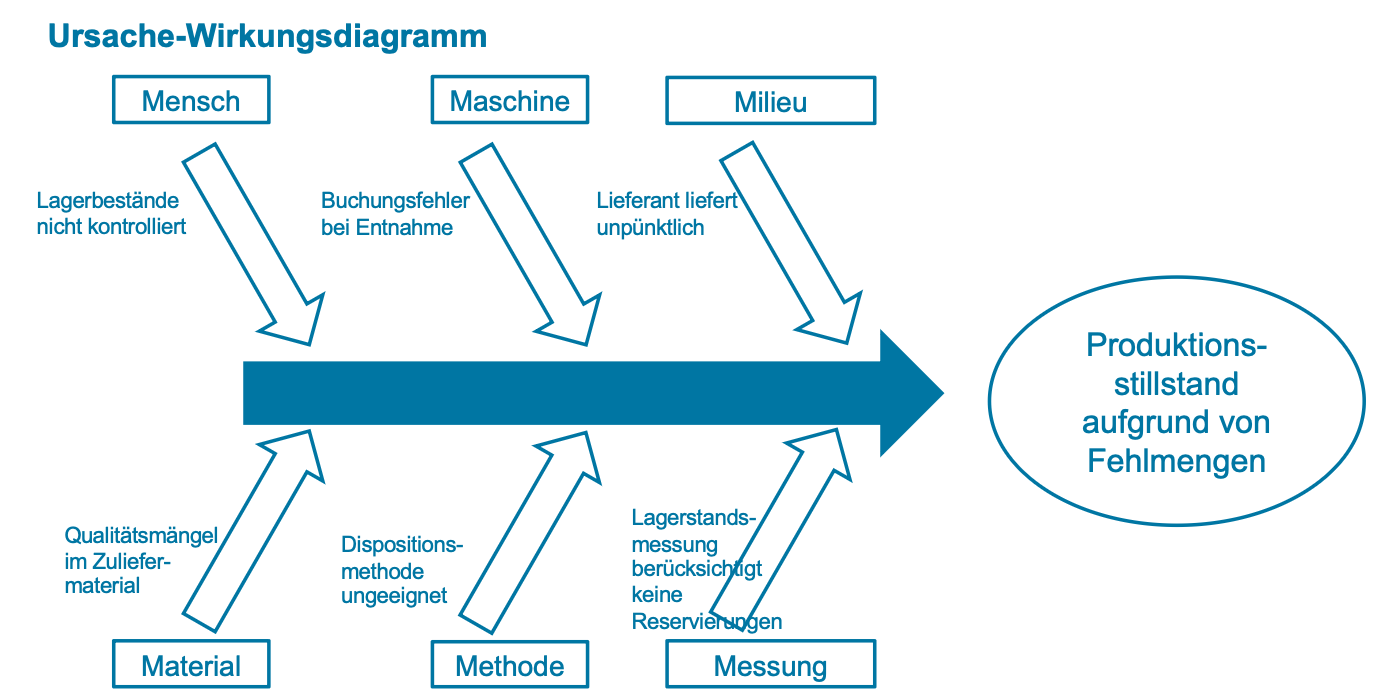
\includegraphics[width=\textwidth]{image/Ursachen-Wirkungsdiagramm.png}
        \caption{Ursachen-Wirkungsdiagramm}
        \label{fig:Ursachen-Wirkungsdiagramm}
    \end{figure}
    \subsubsection*{6M-Methode}
        Identifikation von Ursachen für Prozessprobleme in den Kategorien Mensch, Maschine, Milieu (Prozessumfeld), Material, Methode (Konzeption) und Messung (Daten)
    \subsubsection*{Diagrammerstellung}
        Dokumentation und Klassifizierung der Ursachen in Haupt- und Nebenursachen zur Vorbereitung von Diskussionen

\subsection{Durchlaufzeitanalyse}
    \subsubsection*{Ziel}
        Bewertung der durchschnittlichen Bearbeitungszeit einer Prozessinstanz
    \subsubsection*{Sequenz von Aktivitäten}
        \begin{itemize}
            \item Formel: $DZ_{\text{Sequenz}} = \sum T_i$
            \item Beispiel: Wenn die Durchlaufzeit der Aktivitäten T1, T2 und T3 jeweils 2, 3, 5 Stunden betragen, dann $2+3+5=10$ Stunden
        \end{itemize}
    \subsubsection*{XOR-Block}
        \begin{itemize}
            \item Formel: $DZ_{\text{XOR}} = \sum (p_i * T_i)$
            \item Beispiel: Wenn es zwei Pfade gibt, einer mit einer Wahrscheinlichkeit von 20\% und einer Dauer von 30 Stunden und der andere mit einer Wahrscheinlichkeit von 80\% und einer Dauer von 40 Stunden, dann ist die durchschnittliche Durchlaufzeit $0.2*30+0.8*40=6+32=40$ Stunden
        \end{itemize}
    \subsubsection*{UND-Block}
        \begin{itemize}
            \item Formel: $DZ_{\text{UND}} = T_{\text{parallel}} + max(T_1, T_2, ...)$
            \item Beispiel: Wenn eine parallele Aktivität 10 Stunden dauert und zwei parallele Sequenzflüsse 20 Stunden bzw. 30 Stunden benötigen, dann ist die durchschnittliche Durchlaufzeit $10+max(20, 30)=10+30=40$ Stunden
        \end{itemize}
    \subsubsection*{Wiederholung}
        \begin{itemize}
            \item Formel: $DZ_{\text{Loop}} = \frac{T_{\text{Loop}}}{1-p}$
            \item Beispiel: Angenommen, die Durchlaufzeit für eine Aktivität innerhalb der Schleife beträgt 5 Stunden und die Wahrscheinlichkeit, dass die Schleife wiederholt wird, ist 30\% (also p = 0.3), dann ist die durchschnittliche Durchlaufzeit $\frac{5}{1-0.3}=\frac{5}{0.7} \approx 7,14$ Stunden
        \end{itemize}
    \subsubsection*{Durchlaufzeiteffizienz (DLE)}
        \begin{itemize}
            \item Formel: $DLE = \frac{Bearbeitungszeit}{\text{Gesamte Durchlaufzeit}}$
            \item Beispiel: Wenn die Bearbeitungszeit eines Prozesses 4 Stunden beträgt und die gesamte Durchlaufzeit 10 Stunden ist, dann berechnet sich die Durchlaufzeiteffizienz wie folgt: $DLE= \frac{4 Stunden}{10 Stunden}=40\%$
        \end{itemize}